% Kopfzeile beim Kapitelanfang:
\fancypagestyle{plain}{
%Kopfzeile links bzw. innen
\fancyhead[L]{\Large Vorlesung 2 (17.10.2013)}
%Kopfzeile rechts bzw. außen
\fancyhead[R]{}}
%Kopfzeile links bzw. innen
\fancyhead[L]{\Large Vorlesung 2 (17.10.2013)}
%Kopfzeile rechts bzw. außen
\fancyhead[R]{}
% **************************************************
\chapter{Natürliche Zahlen und vollständige Induktion}\label{P2}
Die vollständige Induktion ist ein wichtiges Beweisprinzip für Aussagen über natürliche Zahlen.\\
Es beruht auf dem...
\section{Induktionsaxiom}\label{2.1}
Sei $M \subseteq \N$ mit
\en{
\item $1 \in M$
\item Für alle $n \in \N$ gilt: $n \in M \Rightarrow n+1 \in M$
}
Dann ist $M=\N$, die Menge der natürlichen Zahlen:\\
$1 \rightarrow 2 \rightarrow 3 \rightarrow \hdots \rightarrow n \rightarrow n+1$

\subsection*{Bemerkung}
Axiome sind grundlegende Aussagen in einer Theorie, die ohne Beweis vorausgesetzt werden.

\section{Satz: Prinzip der vollständigen Induktion}\label{2.2}
Zu jedem $n \in \N$ sei eine Aussage $A(n)$ gegeben. Es gelte:
\en{
\item $A(1)$ ist wahr (Induktionsanfang)
\item Für alle $n \in \N$ gilt: $A(n) \Rightarrow A(n+1)$
}
Dann ist $A(n)$ wahr für alle $n \in \N$\\
``Dominoeffekt'': $A(1)$ ist wahr $\Rightarrow A(2)$ ist wahr $\Rightarrow \hdots$

\subsection*{Beweis}
Setze $M := \{n \in \N : A(n) \text{ ist wahr}\}$\\
$M$ erfüllt 1. und 2. des Induktionsaxioms. Also ist $M=\N$.\\
\qed

\newpage

\phantomsection
\addcontentsline{toc}{section}{Verschiebung des Induktionsanfangs}
\section*{Verschiebung des Induktionsanfangs}
Seien $A(n)$ Aussagen für $n \in \Z$ mit $n \ge n_0$ ($n_0 \in \Z$ fest).\\
Dann gilt das Prinzip der vollständigen Induktion entsprechend mit dem Induktionsanfang bei $n_0$ statt $1$.

\subsection*{Beispiele}
Zuvor: Summen- und Produktzeichen\\
Gegeben seien relle Zahlen $a_k$ für $m \le k \le n$ wobei $m,n \in \Z$ und $m \le n$.\\
Man setzt $\bigsum_{k=m}^n a_k := a_m + a_{m+1} + a_{m+2} + \hdots + a_n$ und $\bigprod_{k=m}^n a_k := a_m \cdot a_{m+1} \cdot a_{m+2} \cdot \hdots \cdot a_n$\\
Konvention für $m>n$ ist:\\
$\bigsum_{k=m}^n a_k := 0$ (leere Summe) und $\bigprod_{k=m}^n a_k := 1$ (leeres Produkt)\\
Oft nützlich: Indexverschiebung, zum Beispiel $\bigsum_{k=m}^n a_k = \bigsum_{k=m-1}^{n-1} a_{k+1}$

\subsubsection*{Beispiel: Arithmetische Summe}
$\bigsum_{k=1}^n k = 1 + 2 + 3 + \hdots + n = ?$ ($n \in \N$)\\
Idee von \href{https://de.wikipedia.org/wiki/Carl_Friedrich_Gau\%C3\%9F}{Carl Friedrich Gauß} für $n=100$ (\emph{Gaußsche Summenformel}):\\
$1+2+3+\hdots+98+99+100 = (1+100)+(2+99)+\hdots+(50+51) = 101 \cdot 50 = 5050$

\section{Satz: Gaußsche Summenformel}\label{2.3}
$\forall n \in \N : \bigsum_{k=1}^n k = \frac{n \cdot (n+1)}{2}$ \emph{(Erinnerung aus dem Vorwort: $\forall$ steht für ``für alle'')}

\subsection*{Beweis mit vollständiger Induktion}
Für ein beliebiges, aber festes $n \in \N$ gelte $A(n)$ $\bigsum_{k=1}^n k = \frac{n \cdot (n+1)}{2}$ \emph{(Induktionsvoraussetzung)}
\en{
\item Induktionsanfang: $n=1$\\
$A(1)$ ist wahr, denn $\bigsum_{k=1}^1 k = \frac{1 \cdot 2}{2} = 1$ \ok
\item Induktionsschluss: $n \rightarrow n+1$\\
Es sei $A(n)$ wahr (Induktionsvoraussetzung, s.o.).\\
$\Rightarrow \bigsum_{k=1}^{n+1} k = \left(\bigsum_{k=1}^n k \right) + (n+1) \iv \frac{n \cdot (n+1)}{2} + (n+1) = (n+1) \cdot \left(\frac{n}{2} + 1 \right) = \frac{(n+1) \cdot (n+2)}{2}$\\
$\Rightarrow A(n+1)$ ist wahr. Mit vollständiger Induktion folgt die Behauptung. \ok
}
\qed

\newpage

\phantomsection
\addcontentsline{toc}{section}{Bemerkung: Rechnen mit Summen (analog für Produkte)}
\section*{Bemerkung: Rechnen mit Summen (analog für Produkte)}
$\bigsum_{k=1}^{n+1} a_k = \bigsum_{k=1}^n a_k + a_{n+1}$\\
Für alle $m \in \N$ gilt: $\bigsum_{k=1}^{n+m} a_k = \bigsum_{k=1}^n a_k + \bigsum_{k=n+1}^{n+m} a_k$

\subsection*{Potenzen}
Sei $x \in \R$ und $n \in \N_0$.\\
Dann: $x^n := \underbrace{x \cdot x \cdot ... \cdot x}_{n \text{ Faktoren}} = \bigprod_{k=1}^n x$\\
Insbesondere: $x^0 = 1$

\section{Satz: Geometrische Summenformel}\label{2.4}
Für $x \in \R \setminus \{1\}$ und $n \in \N_0$ gilt: \fbox{$\bigsum_{k=0}^n x^k = \frac{1-x^{n+1}}{1-x}$}

\subsection*{Beweis mit vollständiger Induktion}
\en{
\item Induktionsanfang: $n=0$\\
$x^0 = 1 = \frac{1-x}{1-x}$ \ok
\item Induktionsvoraussetzung: Für ein beliebiges, festes $n$ gelte: $\bigsum_{k=0}^n x^k = \frac{1-x^{n+1}}{1-x}$
\item Induktionsschluss: $n \rightarrow n+1$\\
$\bigsum_{k=0}^{n+1} x^k \iv \bigsum_{k=0}^n x^k + x^{n+1} = \frac{1-x^{n+1}}{1-x}+x^{n+1} = \frac{1-x^{n+1}+(1-x) \cdot x^{n+1}}{1-x} = \frac{1-x^{n+2}}{1-x}$ \ok
}
\qed

\subsection*{Anmerkung}
Ein Beweis mit vollständiger Induktion setzt voraus, dass man die zu beweisende Identität bereits kennt bzw. vermutet.\\
Eine solche Vermutung gewinnt man z.B. durch Berechnung für kleine Werte von $n$.

\newpage

\phantomsection
\addcontentsline{toc}{chapter}{Binomialkoeffizienten \& Kombinatorik}
\chapter*{Binomialkoeffizienten \& Kombinatorik}

\section{Definition: Fakultät}\label{2.5}
Für $n \in \N_0$ setze $n! = \bigprod_{k=1}^n k = 1 \cdot 2 \cdot \hdots \cdot n$ (sprich: $n$ Fakultät)\\
Also: $0!=1$, $1!=1$, $2!=1 \cdot 2 = 2$, $3!=2 \cdot 3$, $n!=(n-1)! \cdot n$\\
$n!$ wächst sehr schnell, z.B. $13! \approx 6{,}2 \cdot 10^9$\\
Es gibt dafür keine einfache Formel analog zur arithmetischen Summenformel.

\subsection*{Beispiel}
Sei $M=\{a_1 , ... , a_n\}$ eine Menge mit $|M|=n$\\
Wie viele mögliche Anordnungen von $M$ gibt es?\\
$n=2 \Rightarrow M=\{1,2\} \Rightarrow 12, 21 \Rightarrow 2!=2$ Anordnungen\\
$n=3 \Rightarrow M=\{1,2,3\} \Rightarrow 123, 132, 213, 231, 312, 321 \Rightarrow 3!=6$ Anordnungen\\
$n=1 \Rightarrow M=\{1\} \Rightarrow 1 \Rightarrow 1!=1$ Anordnung

\section{Satz: Permutationen}\label{2.6}
Die Anzahl der möglichen Anordnungen \emph{(=Permutationen)}\\
der Elemente einer Menge $M$ mit $|M|=n$ ist $n!$.

\subsection*{Beweis mit vollständiger Induktion}
\en{
\item Induktionsanfang: $n=1$\\
Eine Menge mit einem Element hat genau $1!=1$ Anordnung. \ok
\item Induktionsvoraussetzung: Für ein beliebiges, festes $n$ gelte: $|M|=n \Rightarrow \# \text{Permutationen} = n!$
\item Induktionsschluss: $n \rightarrow n+1$\\
Besetze zunächst die erste Position, dafür gibt es $n+1$ Möglichkeiten.\\
Sei $P_k := \{\text{Permutationen von } 1 , \hdots , n+1 \text{ mit } k \text{ an Position } 1\}$.
Nach Induktionsvoraussetzung ist $|P_k|=n!$ (Anzahl der Möglichkeiten die Stellen $2, 3, \hdots, n+1$ zu besetzen)\\
$\Rightarrow$ Anzahl der Permutationen von $1, 2, \hdots, n+1$ ist $(n+1) \cdot n! = (n+1)!$ \ok
}
\qed

\newpage

\section{Definition: Binomialkoeffizient}\label{2.7}
Seien $k,n \in \N_0$\\
$\bigbin{n}{k} := \bigprod_{j=1}^k \frac{n-j+1}{j} = \frac{n \cdot (n-1) \cdot \hdots \cdot (n-k+1)}{k!}$ (sprich: $k$ aus $n$, oder $n$ über $k$)

\subsection*{Folgerungen}
\en{
\item $\bigbin{n}{0}=1$, $\bigbin{n}{1}=n$, $\bigbin{n}{n}=1$
\item $\bigbin{n}{k}=0$ falls $k>n$
\item $\bigbin{n}{k}=\frac{n!}{k! \cdot (n-k)!}$ falls $0 \le k \le n$
}

\section{Satz: Rekursionsformel}\label{2.8}
$\bigbin{n+1}{k+1} = \bigbin{n}{k} + \bigbin{n}{k+1}$ für $0 \le k \le n$

\subsection*{Beweis}
In der Übung.

\subsection*{Veranschaulichung: Pascalsches Dreieck}
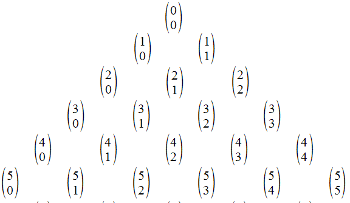
\includegraphics[scale=0.5]{img/2013-10-17/1} $\equiv$ 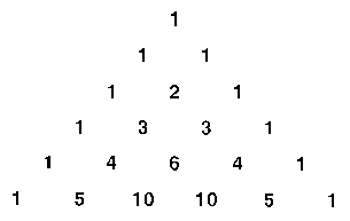
\includegraphics[scale=0.5]{img/2013-10-17/2}

\subsection*{Anmerkung}
Binomialkoeffizienten sind wichtig in der Kombinatorik! \emph{(Stochastik)}

\section{\texorpdfstring{Satz: $k$-elementige Teilmengen}{Satz: k-elementige Teilmengen}}\label{2.9}
Die Anzahl der $k$-elementigen Teilmengen einer $n$-elementigen Menge ist $\bigbin{n}{k}$ ($n \in \N$)

\subsection*{Beispiel}
Beim Zahlenlotto ``6 aus 49'' werden $6$ aus $49$ nummerierten Kugeln gezogen ohne Zurücklegen.\\
Es gibt $\bigbin{49}{6} = 13.983.816$ mögliche Ziehungen.\\
Die Wahrscheinlichkeit für ``6 Richtige'' ist also rund: $\frac{1}{14.000.000}$